\documentclass[english]{article}

\begin{document}


\title{Matrix}
\maketitle
\newcommand{\allezysissi}{allezysissi}
\author{\allezysissi}


\begin{figure*}[h!]
    \centering
    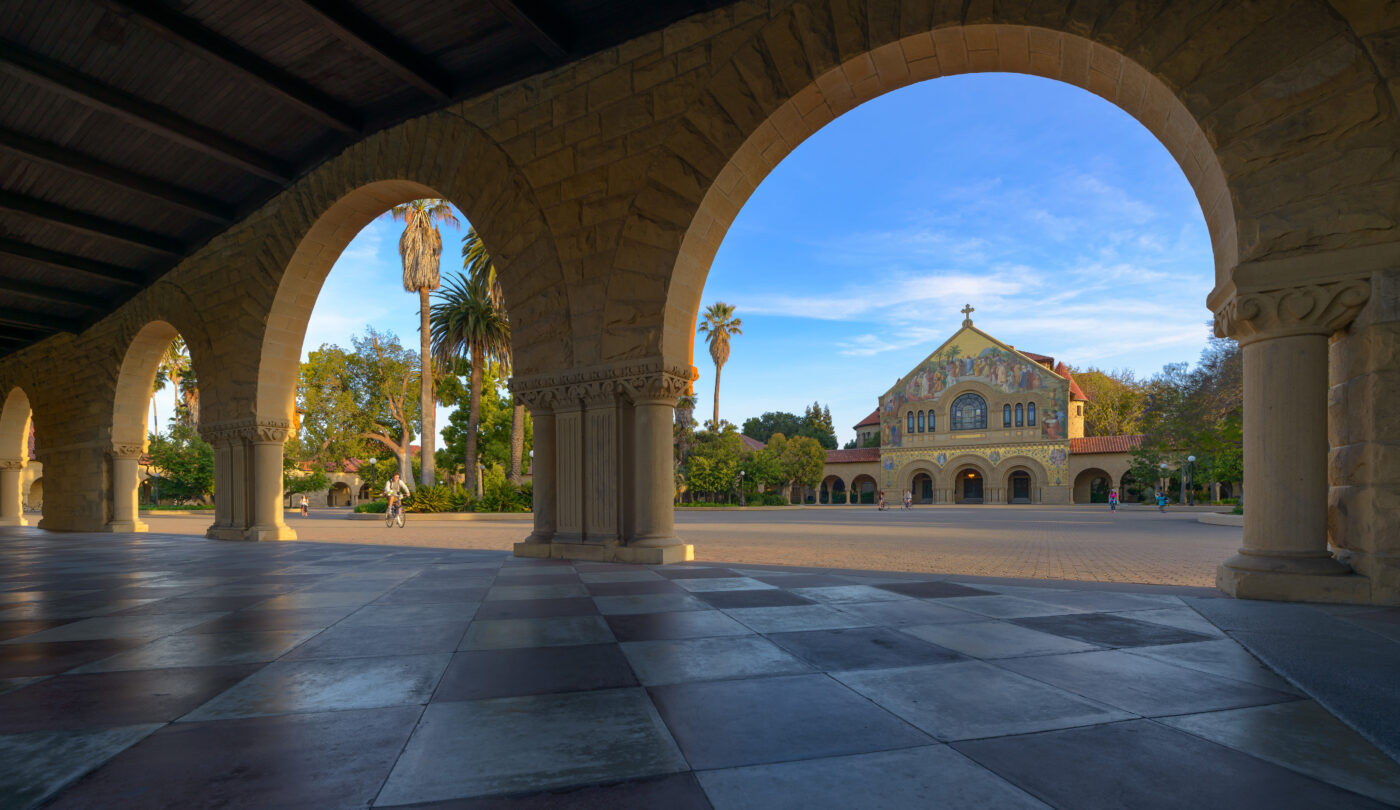
\includegraphics[scale = 0.3]{figs/S.jpg}

    \caption{^}
    \label{fig:S}
\end{figure*}\\
\clearpage

\begin{gather}
 \begin{bmatrix} \lambda_{1} u_{1} & \lambda_{2} u_{2} & \lambda_{3} u_{3}\\ \lambda_{1} v_{1}  & \lambda_{2} v_{2} & \lambda_{3} v_{3} \\ \lambda_{1} & \lambda_{2} & \lambda_{3}
 \end{bmatrix}
 =
 P
  \begin{bmatrix}
   1 & 0 & 0 \\  0 & 1 & 0 \\  0 & 0 & 1 \\  0 & 0 & 0
   \end{bmatrix}
 =
  \begin{bmatrix}
   f & 0 & x_{0} \\  0 & f & y_{0} \\  0 & 0 & 1
   \end{bmatrix}
   R
\end{gather}

Ax=b\\

f = \sqrt{-(u_{1}-x_{0})(u_{2}-x_{0})-(v_{1}-y_{0})(v_{2}-y_{0})}\\

\begin{gather}
K 
=
\begin{bmatrix}
   f & 0 & x_{0} \\  0 & f & y_{0} \\  0 & 0 & 1 
   \end{bmatrix}
   \end{gather}


\end{document}
